\chapter{Indoor flooring}

	\section{flooring typology}
	
	Indoor flooring or paving is the horizontal base of a building (or the different bases of each building level). It works as a support for people or furniture. Indoor paving can be provided with several types of coating (wood, ceramics, marble, et cetera).
	
	The coating material is the first thing to be decided before choosing any other feature of the floor, such as color, texture or specific details.
	
	In general, the most common used materials in flooring are: wooden floors, ceramic floors, petrous floors and those made of concrete. There are also other materials, such as metallic and artificial composite floors, although these are less common.
	
	Depending on the application that is going to be given to the floor, or the indoor zone in which is going to be set up, one must take into account the following aspects:
	
	\begin{itemize}
	\item \textbf{Wear and tear resistance}: it is advised to use ceramic floors, petrous or concrete. For example, in circulation areas or stairs.
	
	\item \textbf{Perforation resistance}: some concretes with specific resistances, some petrous or ceramic floors. 
	
	\item \textbf{Humidity resistance}: ceramic, petrous and ceramic offer a high humidity resistance; on the other hand, wooden floors are not recommended. To be taken into account in restrooms or rainy areas.
	
	\item \textbf{Resistance to chemicals}: some kind of petrous floors such as granite and specific ceramics. In zones where chemical pourings can happen.
	
	\item \textbf{Hygiene}: the floor must have the ability of being easily cleanable and waterproof, to show an attractive and newflanged aspect.
	\end{itemize}
	
	To back up the decision that has been made, some general features of each floor type are presented next:
	
	\begin{itemize}
	\item \textbf{Wooden floors}: 
	Nowadays, and thanks to the advanced wood treatments, it is possible to find dyed and varnished wooden floors. These kind of floors can last up to 50 years. They add warmness to cool places; and with a proper setting and maintenance they can remain as untouched during several years. Among their disadvantages, it is found that they require special care for cleaning and mantaining and also they can be deteriorated with humidity or water pouring. Wooden floors can be natural, synthetic or laminated. These floors are more common in Europe.
	
	\item \textbf{Ceramic stoneware or porcelain stoneware floors}:
	These kind of floors have a decent price according to its usage. The average lifetime of a stoneware tile is of about 30 years. Naturally, they have low resistance to wear due to material properties, although the can be restructured to increase resistance.
	
	\item \textbf{Petrous floors}: 
	Different kind of stones are used in flooring: marble, slate, granite, quartz, sandstone, etc. Their main advantage is the wear resistance. This resistance is greater than for ceramic stoneware floors. Due to the attractive patterns and high resistivity properties, these materials can be the most expensive.
	
	Regarding marble pavings, this material denotes nobility and it was usually used for paving prestigious places. Its main features are its aspect and resistance; its disadvantages are the coldness to touch, and the necessity of a high maintenance to avoid imperfections.
	
	Other rocks used in paving are quartz, slate and granite, being the lattest much resistant than marble, but very expensive to cut, prepare and set into the floor.
	
	\item \textbf{Vinyl floors}:
	Vinyl floors are easy to clean, they also resist humidity and water pourings. They are easy to replace and to set above other floor coatings. This kind of floors are thermic and electrical insulators. Among their disadvantages, they look artificial and need a careful and correct use to avoid imperfections.
	
	\item \textbf{Smooth concrete floors}:
	This kind of floors are easy to maintain and offer resistance. Drawings, shapes and colors can be designed on it. A proper instalation leads not only to a good appearance but also to a greater resistance avoiding wear and fissures.
	
	\item \textbf{Brick floors}:
	Brick floors are economic, providing a rustic decoration or also common in exteriors, they offer a high sensitivity to attrition and show wear in heavily-transited areas.
	
	\item \textbf{Carpet floors}:
	They are quite economic and of easy instalation, without the need of hiring specialized personnel. Like wooden floors, carpet is available in different colors and patterns and provides warmness, and add aesthetics in the place used. It insulates sound and temperature. Its main disadvantage is the accumulation of dust, and therefore it requires a constant maintenance. Carpet floors are very common in the U.S., specially in public places such as airports.
	\end{itemize}
	
	\section{Floor covering}
	
	In any paving, before setting the upper finishing layer, which is different depending upon the zone, it is important to know the layers that have to be included in-situ:
	\begin{itemize}
	\item Surface layer 
	\item Grip layer 
	\item Leveling layer 
	\item No-grip intermediate layer 
	\item Structural base 
	\end{itemize}
		\subsection{Structural base}
	The structural base is the layer that lies onto the floor. In the particular case of indoor paving, it is formed by a ground slab.
	
	Ground slabs, also knowns as floor framings, are classified in terms of stability as a consequence of hydraulic retention, according to the normative UNE 22202-1.
	
	The thickness of the ground slabs is determined by means of structual criteria, as functions of the CBR (California Bearing Ratio). On the other hand, a solicitation computation is also required.
		\subsection{No-grip intermediate layers}
		
	To enhance the floor properties different layers composed by different materials are inserted. These layers are the following ones:
	\begin{itemize}
	\item Waterproof layer: this layer raincoats the floor against liquid water. It is recommended to use a polyethylene layer of a minimum thickness of 2mm. 
	\item Drainage layer: it helps removing the water that might be stored by means of a small slope. 
	\item Acoustic insulation: there are specific layers for this function, and it helps insulate and reduce the impact of aerial noise, which is spread within the structure.
	\item Thermal insulation: it enchances a greater thermal resistance.
	\end{itemize}
		\subsection{Leveling layer}
	These kind of layers are used to achieve the required flatness of the firm, and if a certain slope is required, they also provide this slope.
		\subsection{Grip layer}
	It consitutes the union between structural base and the tile or coating. It can be made of a leveling mortar or an adhesive. In the project, a leveling mortar has been chosen.
		
	\section{Design}
	The floor design and aesthetics is wanted to produce a homely and cozy feeling. In order to do so, it has been thought that it could fit with the tonalities of the landscapes that can be seen all across the country, and the beautiful sceneries that are spread along the islands and towns of Indonesia.
	
	There is a lot of culture of esculptures in the islands of Java and Bali, for this reason, a floor design that reminds of the ancient sculptures of the country could fit in the airport and also provide a clean, elegant and cozy appearance.
	
	\begin{figure}[ht!]
	\centering
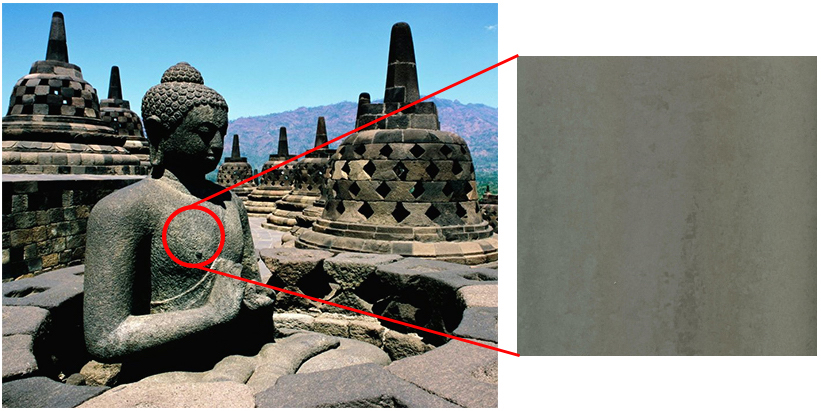
\includegraphics[width=13cm]{./images/SueloGeneral}
\end{figure}

On the other hand, an inspiration from the beautiful and relaxing beaches that the country offers, it has been chosen a floor that reminds of the sand that one can find in these beaches.

\begin{figure}[ht!]
	\centering
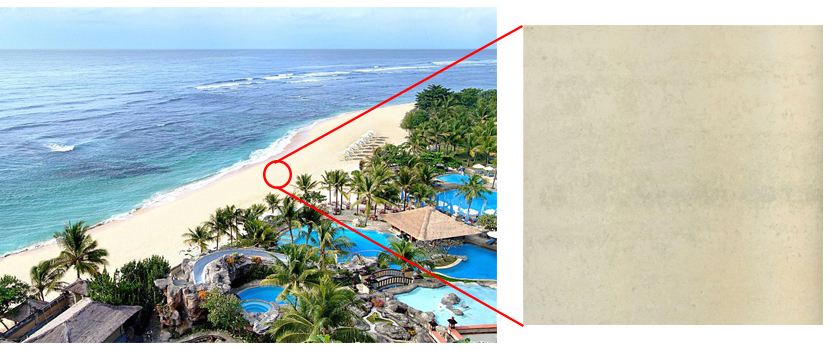
\includegraphics[width=15cm]{./images/SueloSecundario}
\end{figure}

	
	
	
	\section{Superficial layer}
		\subsection{Common areas flooring}
	In the common areas, it has been chosen to use a ceramic porcelain stoneware Floor Gres material, in particular the technical strong collection Chromtech/1.0 from the Floor Gres company, that is suitable for heavy traffic areas thanks to its high resistance. The color will be a neutral grey named cool/3.0 in the Floor Gres company color gamma.
	
	\begin{table}[ht!]
	\centering
	\begin{tabular}{|c|c|c|}
	\hline
	Specification & Normative & Value\\
	\hline
	Water Absorption & ISO 10545-3 & $<0.1\%$\\
	\hline
	Breaking Strength & ISO 10545-4 & $>1700$ N\\
	\hline
	Scratch Hardness & ISO 10545-6 & $< 150 \mathrm{mm^3}$\\
	\hline
	Thermal Shock Hardness & ISO 10545-9 & Resistant\\
	\hline
	Chemical Resistance & ISO 10545-13 & UA ULA UHA\\
	\hline
	Coefficient of Friction & DIN 51130 & R10 (Matte)\\
	\hline
	\end{tabular}
	\caption{Technical Specs of Floor Gres Chromtech/1.0 floor.}
	\end{table}
	
The color chosen for our tiles within all the color shades is the one known as "Cool 3.0" with a matte and polished finishing.
	\begin{figure}[ht!]
	\centering
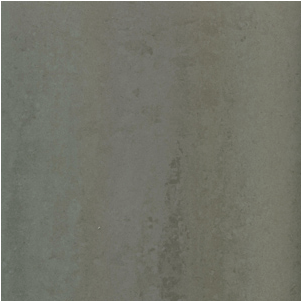
\includegraphics[width=1cm]{./images/Color}
\caption{Neutral gray color (Cool 3.0) from Floor Gres gamma.}
\end{figure}

The result of the floor chosen in the common areas is the following:
\begin{figure}[ht!]
	\centering
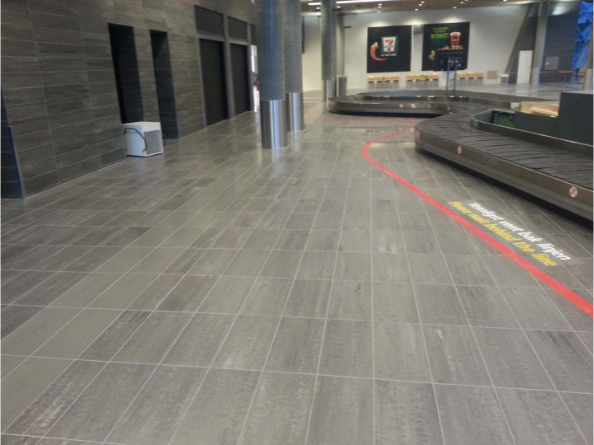
\includegraphics[width=10cm]{./images/Resultado}
\caption{Result of instaling Chromtech/1.0 tiles in common areas.}
\end{figure}
		\subsection{Stairways and secondary areas flooring}
	Due to the high-end properties provided by the floor used in the common areas, it has been decided to use the same material but with a different tonality. In this case, the color chosen is  a beige/taupe named Cool 1.0 in the Floor Gres color gamma. It is provided with a matte finishing.
	
	The technical specs of these tiles are the same as for the tiles used in common materiales provided that the only change is the color. In general, this product provides an excellent finishing and it offers a high resistance. For this reason, it can be used in heavily-trafficked areas.
	
	The color that has been chosen for stairways and secondary areas such as VIP lounges is the following:
		\begin{figure}[ht!]
	\centering
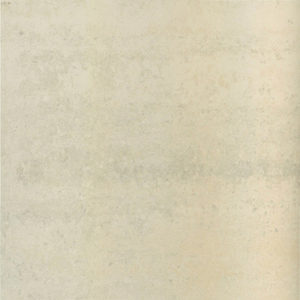
\includegraphics[width=1cm]{./images/Color2}
\caption{Beige/taupe color (Cool 1.0) from Floor Gres gamma.}
\end{figure}

The result of the floor chosen in stairways and secondary areas is the following:
\begin{figure}[ht!]
	\centering
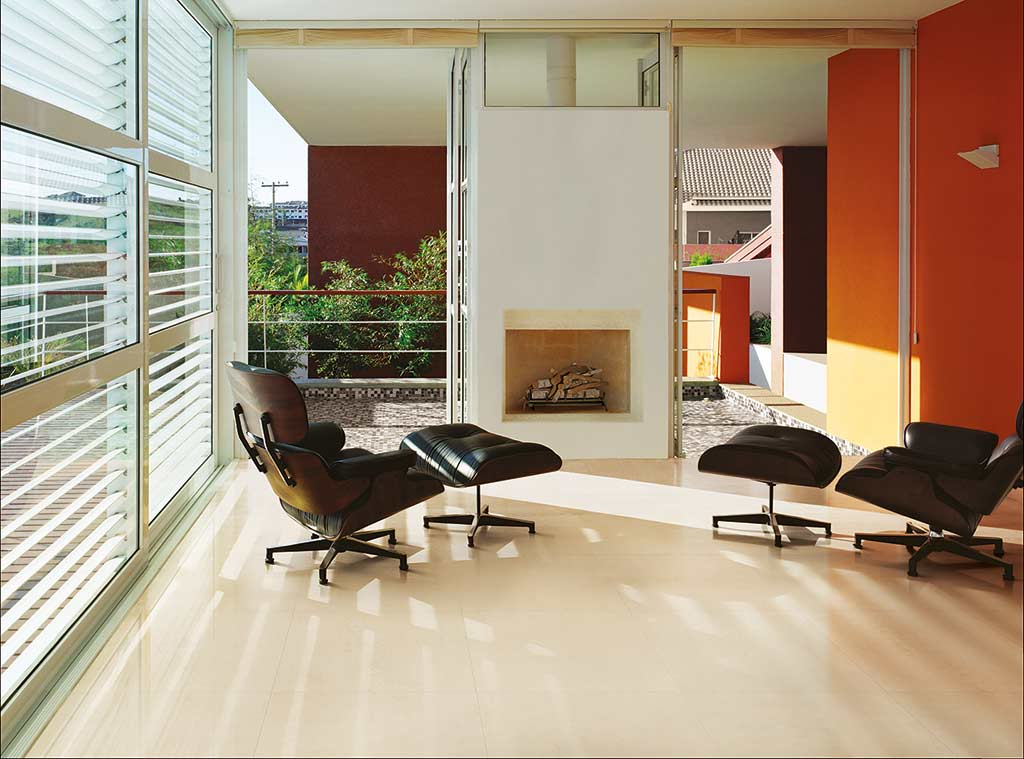
\includegraphics[width=10cm]{./images/Resultado2}
\caption{Result of instaling Chromtech/1.0 tiles in secondary areas.}
\end{figure}
		\subsection{Restrooms flooring}
	For the restrooms paving, it has been decided to use a rectified porcellanato tile, named "Portland Caliza" from the Spanish company Porcelanosa. These tiles are provided with anti-slip properties, making them exceptional for the usage in restrooms.
	
	The color chosen is called "colored biscuit" and it is a neutral light gray:
			\begin{figure}[ht!]
	\centering
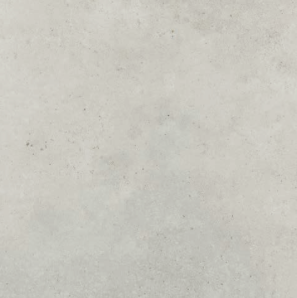
\includegraphics[width=1cm]{./images/Color3}
\caption{Neutral light gray "Colored Biscuit" from Porcelanosa.}
\end{figure}

The result of instaling these tiles in the airport restrooms is the following:

\begin{figure}[ht!]
	\centering
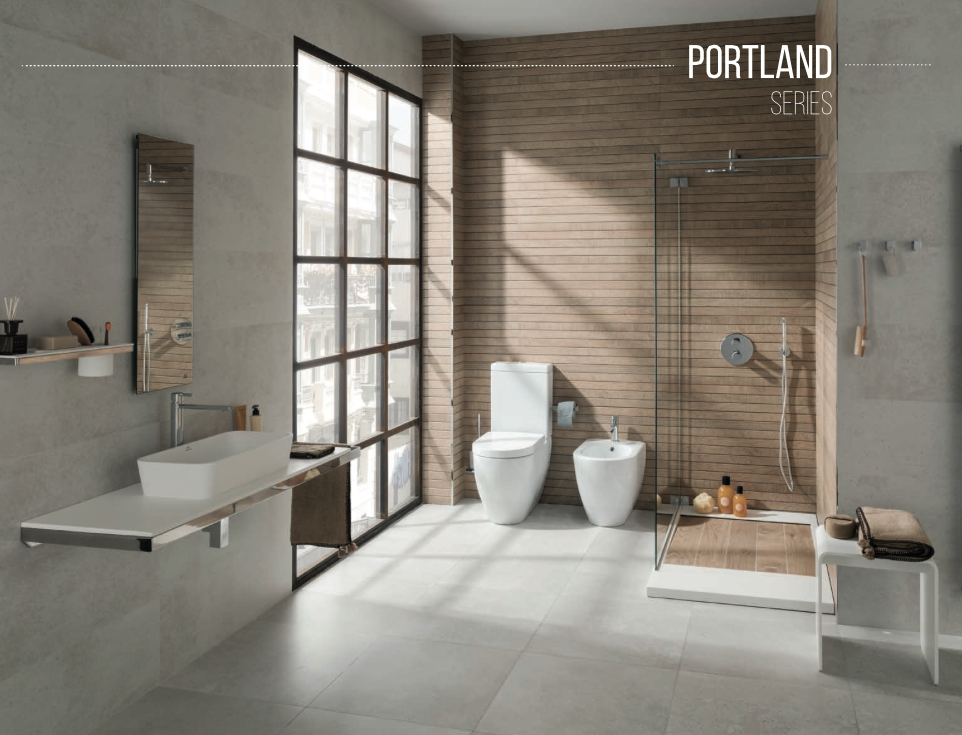
\includegraphics[width=8cm]{./images/Resultado3}
\caption{Result of instaling Portland Caliza tiles in restrooms.}
\end{figure}
	
		\subsection{Offices flooring}
	The airport offices for ANSPs, customs and airlines are going to be provided with a porcelain stoneware tile called Basalike from a company called Panaria. The supply of these tiles is to be provided by the Italian company Sognando Casa, that manufactures several types of materials for indoor flooring.
	
	These tiles offer an excellent natural finishing with an antislip index R10. The color chosen is a dark gray that inspires calmness and make the offices the perfect spot for working in any season of the year.
	
	The color that will be instaled in the offices floor is the following:
\begin{figure}[ht!]
\centering
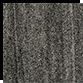
\includegraphics[width=1cm]{./images/Color4}
\caption{Dark gray color in Basalike tiles from Panaria company.}
\end{figure}

The result of instaling these tiles in the airport offices is the following:
\begin{figure}[ht!]
	\centering
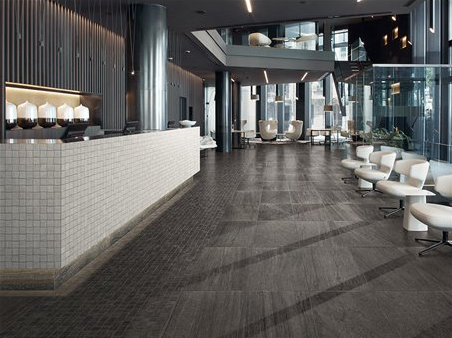
\includegraphics[width=10cm]{./images/Resultado4}
\caption{Result of instaling Basalike tiles in the airport offices.}
\end{figure}

These tiles have good quality and are optimum for an office flooring. In the next table, the technical specifications are shown:

	\begin{table}[ht!]
	\centering
	\begin{tabular}{|c|c|c|}
	\hline
	Specification & Normative & Value\\
	\hline
	Water Absorption & ISO 10545-3 & $<0.5\%$\\
	\hline
	Breaking Strength & ISO 10545-4 & $>1300$ N\\
	\hline
	Scratch Hardness & ISO 10545-6 & $< 175 \mathrm{mm^3}$\\
	\hline
	Chemical Resistance & ISO 10545-13 & LA, HA\\
	\hline
	Coefficient of Friction & DIN 51130 & R10 (Natural)\\
	\hline
	\end{tabular}
	\caption{Technical Specs of Panaria Basalike floor.}
	\end{table}
	
		\subsection{Automatic baggage handling system flooring}
		
	The automatic baggage handling system flooring is not so much sophisticated and for obvious reasons, ceramic or porcelanic tiles will not be used. In this area, polished concrete is to be used since it provides a set of good properties for this application:
	\begin{itemize}
	\item High surface mechanical resistance.
	\item Greater useful life than conventional concrete.
	\item High density and low porosity.
	\item Easiness of maintenance and cleaning.
	\item Low dust formation.
	\end{itemize}
The supplying of the concrete and its respective polishing will be provided by the Spanish company EIROS, since it offers a good service at a honest price.

\begin{figure}[ht!]
	\centering
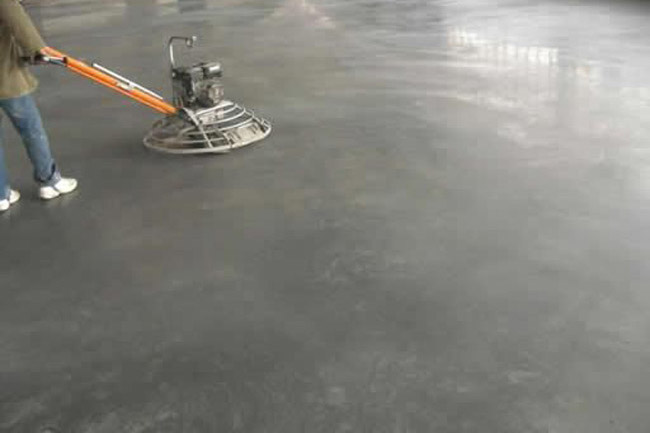
\includegraphics[width=10cm]{./images/Resultado5}
\caption{Result of instaling polished concret in the ABHS system (SATE).}
\end{figure}

		